\documentclass[11pt,a4paper]{article}
\usepackage[T1]{fontenc}
\usepackage[utf8]{inputenc}
\usepackage{lmodern}
\usepackage[margin=2.35cm]{geometry}
\usepackage{setspace}
\setstretch{1.05}
\usepackage{amsmath,amssymb,booktabs}
\usepackage{graphicx}
\usepackage{siunitx}
\sisetup{detect-weight=true,detect-family=true}
\DeclareSIUnit{\ppb}{ppb}
\usepackage[numbers,sort&compress]{natbib}
\usepackage{microtype}
\usepackage[hidelinks]{hyperref}
\setlength{\parskip}{0.28em}
\setlength{\parindent}{1.05em}
\usepackage{caption}
\captionsetup{font=small,skip=4pt}

\title{A Physics-Informed Pressure Digital Twin\\ for a High-Gravity Beer Blend Skid}
\author{Department of Computer Science}
\date{October 2026}

\begin{document}
\maketitle
\begin{abstract}
\noindent
A nonlinear predictive controller for high-gravity blending is only as good as the valve capacities and the header pressure it believes. This paper builds a physics-informed pressure digital twin of the three-valve blend network. A commissioning campaign of twenty-eight noisy steady points estimates the three valve capacities and a beer-header pressure bias to well inside one percent. Pipe roughness and the lumped minor-loss coefficient are not separately identifiable; their sum, an effective line loss, is recovered to about two and a half percent. A residual network with a mass-balance penalty is trained on the same campaign and then gated off, because the hold-out flow error rises from \SI{0.030}{\cubic\metre\per\hour} to \SI{0.037}{\cubic\metre\per\hour}. Deployed as the model inside the predictive controller, the calibrated physical twin brings a lager-to-light grade change inside \SI{0.05}{\degree}P in \SI{16}{\second}. The same controller on the uncommissioned model leaves an offset of about \SI{0.19}{\degree}P. The twin also inverts a measured water-valve deadband. It does not, and cannot, remove dissolved oxygen that arrives in the dilution water.
\end{abstract}

\section{Introduction}
A digital twin is a model kept aligned with a particular asset and used for a decision \citep{kritzinger2018}. In brewing, published twins have been built around fermentation sampling and monitoring \citep{goffi2025}. The blend skid is a different asset. Its decision is a valve move on a time scale of seconds, and the parameters that move the beer are hydraulic: three capacities $K_v$, a possible bias on the beer-header transmitter, and the friction loss of the blend line. A predictive controller that uses the wrong capacities asks for the wrong lifts. A ratio station is less exposed, because its flow loops close on measured flow. The twin exists so that the predictive controller is entitled to its model.

Hybrid models and physics-informed networks are the usual way to attach data to a balance \citep{vonstosch2014,raissi2019,karniadakis2021}. Process applications keep the network when the hold-out improves and use the corrected model inside predictive control \citep{zheng2023,wu2023cerd}. The rule adopted here is the same rule with the opposite deployment: the network is kept only if the hold-out flow error falls. On this skid it rises, and the deployed twin is the calibrated valve law alone.

\section{What the flows can identify}
The valve law is the installed form of IEC~60534 \citep{iec60534},
\begin{equation}
Q = K_v\,50^{\,l-1}\sqrt{\frac{\Delta p}{\rho/1000}}.
\end{equation}
The blend line adds a Darcy loss. At a fixed Reynolds number that loss depends on roughness $\varepsilon$ and on the minor-loss coefficient $K$ only through
\begin{equation}
C_L = f(\varepsilon)\,L/D + K.
\end{equation}
A positive step in $\varepsilon$ and a compensating step in $K$ leave $C_L$, and therefore every flow, unchanged. The two columns of the residual Jacobian are then scalar multiples, and the formal standard errors diverge. The engineering parameter is $C_L$. The campaign reports that sum and withholds a roughness.

Capacities do not share a column. $K_{v,h}$ scales only the beer flow, and a change of beer lift changes the drop and the flow in a combination that a pure header bias cannot imitate. The beer-header bias $b_h$ is therefore estimated jointly with the three capacities, by nonlinear least squares on steady points. Twenty-eight points are used, with flow noise of about \SI{0.03}{\cubic\metre\per\hour} and pressure noise of \SI{0.008}{bar}. The header reading is high by \SI{0.10}{bar} until the bias is removed. The true line is $C_L=18.85$, from a Haaland friction factor at $\varepsilon=\SI{2}{\micro\metre}$ plus $K=14$ \citep{crane2009}.

Two further scalars are not in that regression. The solubility scale $\kappa_\zeta$ is a single bench point relating dissolved carbon dioxide to equilibrium pressure. The density contraction $\gamma$ in $\rho\propto(1-\gamma A_w E_r)$ is the median of Coriolis densities. Both are identifiable from measurements the flow campaign does not contain, and both are recovered to the plant values.

\begin{table}[t]
\centering
\caption{Commissioning estimates. Standard errors are from the linearised least-squares covariance. Roughness and minor loss are omitted as a pair; the table publishes their sum $C_L$.}
\label{tab:est}
\begin{tabular}{lrrr}
\toprule
Parameter & True & Estimate & Std.\ error \\
\midrule
$K_{v,h}$ (m$^3$/h) & 32.00 & 32.02 & 0.08 \\
$K_{v,w}$ (m$^3$/h) & 12.00 & 12.00 & 0.01 \\
$K_{v,f}$ (m$^3$/h) & 64.00 & 63.99 & 0.12 \\
Header bias (bar) & 0.100 & 0.098 & 0.006 \\
Effective loss $C_L$ & 18.85 & 18.37 & --- \\
Solubility scale $\kappa_\zeta$ & 0.930 & 0.930 & --- \\
\bottomrule
\end{tabular}
\end{table}

Table~\ref{tab:est} is the result. The capacity errors are a few hundredths of a cubic metre per hour on valves of capacity $12$ to $64$. The bias error is \SI{0.002}{bar}. The effective loss is about \SI{2.5}{\percent} low. That is accurate enough for the grade change in Section~\ref{sec:loop}. It is not a licence to publish $\varepsilon=\SI{2}{\micro\metre}$ as an identified roughness. A later campaign should estimate $C_L$ directly.

\section{The residual network and the gate}
Let $\xi$ be the standardised feature of the three lifts, the two mother-beer analyses and the mix pressure. A network with eight hidden units predicts a flow correction,
\begin{equation}
h = \tanh(W_1\xi+b_1),
\qquad
\Delta Q = W_2 h + b_2,
\end{equation}
with $W_1\in\mathbb{R}^{8\times 6}$ and $W_2\in\mathbb{R}^{3\times 8}$. Training minimises the squared residual against the measured flow error, plus weight decay, plus a penalty on $\Delta Q_h+\Delta Q_w-\Delta Q_f$ every fifth step. The penalty is the mass balance the three flows already obey. It is not a collocation residual of a partial differential equation \citep{raissi2019}.

Six points are held out. Root-mean-square flow error on those points is \SI{0.0296}{\cubic\metre\per\hour} for the physical model and \SI{0.0365}{\cubic\metre\per\hour} after $\Delta Q$ is added. Eight hidden units on twenty-two training points are enough capacity to fit the noise of a residual that is already at the sensor floor. The gate compares the two errors and publishes the physical prediction. The weights stay on disk with the campaign so that a later campaign can be scored against the same architecture. They are not written into the controller. Figure~\ref{fig:parity} is the flow parity of the physical twin.

\begin{figure}[t]
\centering
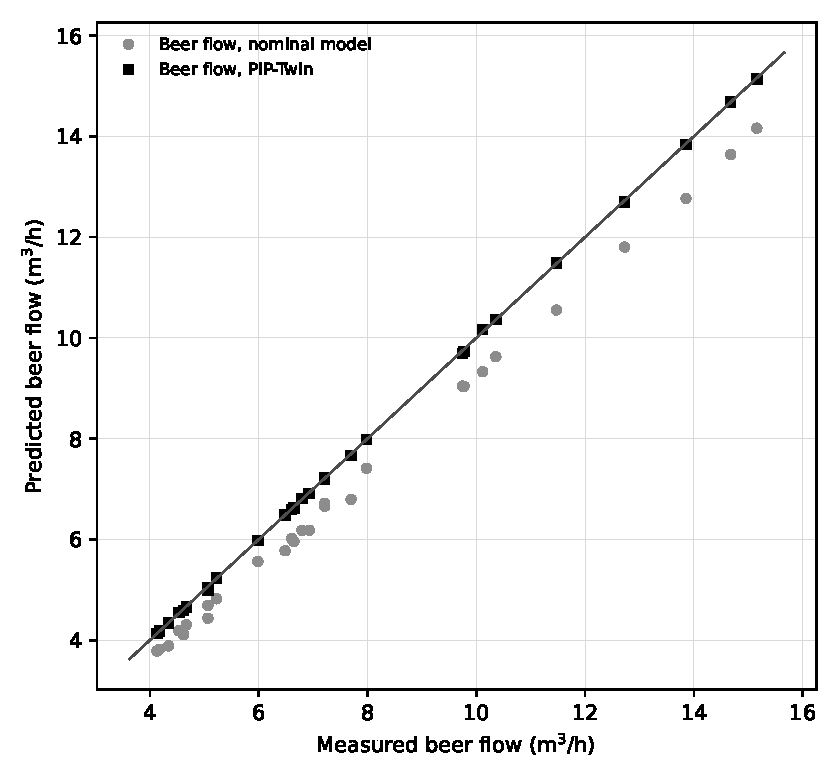
\includegraphics[width=0.62\textwidth]{../main/figures/parity_flow.pdf}
\caption{Commissioning parity of predicted and measured flow for the calibrated physical model. The residual network is not added.}
\label{fig:parity}
\end{figure}

The same campaign records a water-valve deadband when a command changes and the stem does not \citep{choudhury2005,jelali2010}. If the band width $S$ is known, the command is led by $S$ in the direction of the requested move, so the stem crosses the band and the flow that appears is the flow the brand asked for. Undetected, the same band turns a small flow correction into a delayed jump.

\section{Closed-loop consequence}
\label{sec:loop}
The consumer of the twin is a three-valve nonlinear predictive controller. Two copies are run. One uses the nominal model: capacities $29.4$, $13.2$ and $58$, a rougher pipe, no density contraction, and a header bias of $+0.10$ bar that the model believes. The other uses Table~\ref{tab:est}, with the bias removed from the header measurement. The ratio station does not use either model for its flow loops. All three see the same sensor noise.

On a lager-to-light grade change the commissioned controller is inside \SI{0.05}{\degree}P at \SI{16}{\second}, with an extract integral of \SI{10.75}{\degree}P$\cdot$s and a tail of $+\SI{0.012}{\degree}P$. The nominal controller's extract integral is \SI{32.29}{\degree}P$\cdot$s, statistically the same as the ratio station's \SI{31.30}{\degree}P$\cdot$s, and its tail is $+\SI{0.19}{\degree}P$. The horizon, the weights and the rate limit are identical. The difference is the parameter vector. An uncommissioned predictive controller is the expensive choice.

On a mother beer that cannot hit extract and alcohol together, the commissioned tail matches the tolerance-weighted optimum computed offline: \SI{11.777}{\degree}P and \SI{4.695}{\percent} by volume against \SI{11.780}{\degree}P and \SI{4.696}{\percent} by volume. The nominal controller, following a biased gain, sits elsewhere. The twin does not create a feasible point that the mother beer does not allow. It makes the compromise the one the tolerances define.

On a sticky water valve of band $0.03$ lift, the twin learns the band after \SI{8}{\second} and leads the command. The extract integral is \SI{1.29}{\degree}P$\cdot$s and the error stays inside \SI{0.05}{\degree}P. The nominal controller, with the wrong gain and no deadband inverse, has an extract integral of \SI{19.28}{\degree}P$\cdot$s. The ratio station, closing on measured flow, has \SI{3.97}{\degree}P$\cdot$s. When the same run raises dilution-water oxygen from \SI{12}{ppb} to \SI{85}{ppb}, every controller's product reaches about \SI{31}{ppb}. The twin reports that concentration. No valve move removes it.

\section{Conclusion}
The innovation is a pressure twin whose parameters are the ones the blend flows can actually see, together with an explicit refusal to deploy a residual correction that fails the hold-out. Valve capacities and the header bias are identified to a fraction of a percent. Roughness and minor loss are identified only as the sum $C_L$, to about two and a half percent. The residual network is part of the method because the gate is part of the method: the correct action on this campaign is to leave it off. Used as the model of a three-valve predictive controller, the twin is what turns a program that ties ratio control into a program that meets a feasible brand change in \SI{16}{\second} and an infeasible brand at the weighted compromise. The study commissions a simulated skid whose equations the estimator already knows in structure. A trim that is not equal-percentage, or a mixer that is not one volume, would be a reason to reopen the gate on new step tests. It would not be a reason to skip the hold-out.

\bibliographystyle{unsrtnat}
\bibliography{refs}
\end{document}
